\chapter{热辐射}\label{ch:b2:thermal-radiation}

一切温热的物体都会发光。手、墙壁、室温下的一杯水，
都会辐射波长接近 \qty{10}{\micro m} 的、人眼看不见的电磁波，
每平方米辐射功率约为几百瓦；把一根火钳加热，
到 \qty{600}{\celsius} 时呈暗红色，到 \qty{1000}{\celsius} 时变橙，
到 \qty{2500}{\celsius}（即灯泡灯丝的温度）时发出白光；
太阳表面温度为 \qty{5800}{K}，发出黄白色的光，
每平方米辐射功率约为六十兆瓦；这束光经过八分钟到达地球，
使地球保持在水能呈液态的温度。辐射是热传递的第三种方式，
也是唯一能穿越真空的方式。
正是在辐射问题上，经典物理遇到了困难：普朗克
于 1900 年不得不引入量子假设。本章给出他所得到的定律，
由此导出两个常用结果——
维恩位移定律与斯特藩–玻尔兹曼定律，
并将它们应用于物体之间的热交换、太阳与地球，
以及决定我们气候的单层温室效应模型。

\begin{omfigure}
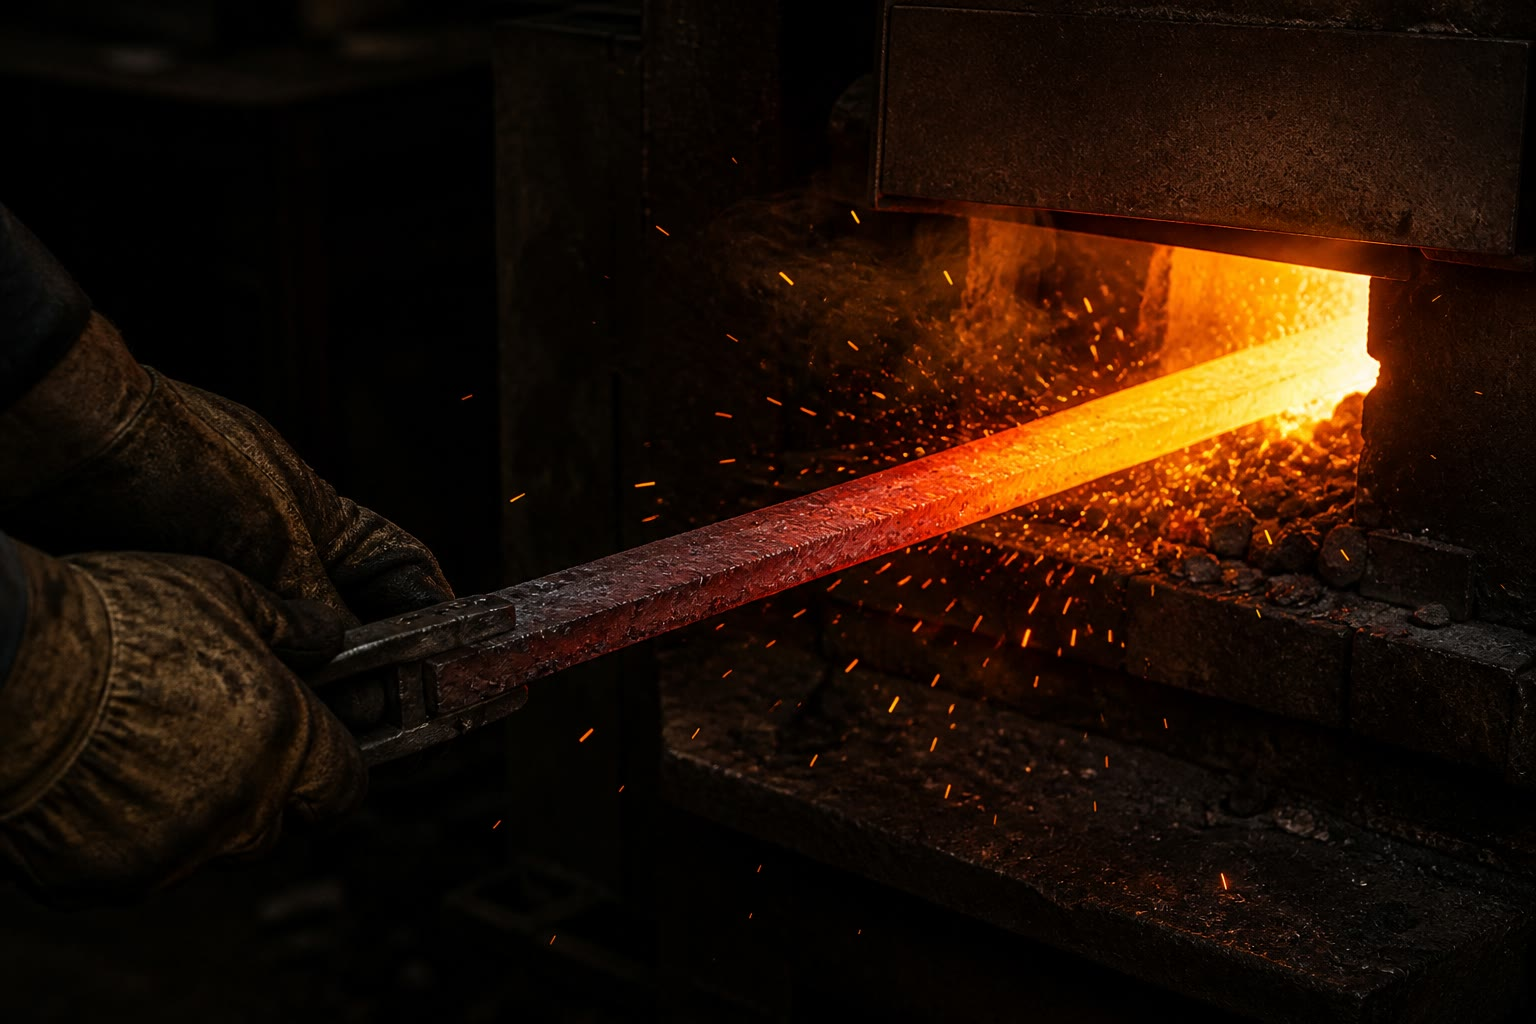
\includegraphics[width=0.58\linewidth]{images/book4/ai/b4-26-glowing-steel-forge.jpg}

{\small 锻炉中的钢件：发光的颜色——暗红、橙、黄、白——就是一支温度计，
因为热辐射的光谱只由温度决定，
与其他因素无关。}
\end{omfigure}

\section{热辐射与黑体}

\begin{definition}[热辐射、吸收率、黑体]\label{def:b2:thermal-radiation:blackbody}
温度为 $T$ 的每个物体，都会因其电荷的热运动而发射电磁辐射，
这种辐射称为\emph{热
辐射}\index{热辐射}。物体表面还接收来自外界的辐射，
并吸收其中的一部分，吸收的比例记为 $\alpha$，
（即\emph{吸收率}，介于 $0$ 与 $1$ 之间，一般依赖于波长），
其余部分则被反射或透射。若物体吸收全部入射辐射，则称之为\emph{黑
体}\index{黑体}，即对每个波长都有 $\alpha = 1$。
闭合空腔壁上的一个小孔是黑体的
实际模型：射入小孔的辐射在能逸出之前，
就已在腔壁上被吸收。
\end{definition}

\begin{proposition}[平衡辐射与基尔霍夫定律]\label{prop:b2:thermal-radiation:kirchhoff}
在壁温为 $T$ 的闭合空腔内，辐射与腔壁处于平衡，
并且是\emph{普适的}：各向同性、无偏振，
其谱能量密度 $u_\nu(T)$（单位体积、单位频率内的能量）
仅依赖于 $T$ 与 $\nu$，而与空腔的材料和形状无关。
从这种空腔的小孔射出的辐射，
即温度为 $T$ 的\emph{黑体辐射}。
若一个表面在某一频率下吸收其所接收辐射的比例为 $\alpha_\nu$，
则它在该频率 $\nu$ 处发射的
为同温度黑体所发射量的比例 $\varepsilon_\nu = \alpha_\nu$（其
\emph{发射率}\index{发射率}）；
即\emph{好的吸收体也是好的发射体}。
\end{proposition}

\begin{proof}
普适性：将两个温度同为 $T$ 的空腔
用一个只让单一频率通过的滤光片的小孔相连；若两者能量密度不同，
则在相同温度下能量将从一个空腔流向另一个，
这违背热力学第二定律。基尔霍夫：将物体置于其自身温度 $T$ 的空腔内；
处于平衡时，它在每个频率上发射的能量必须恰好等于其吸收的能量，
即 $\varepsilon_\nu u_\nu = \alpha_\nu u_\nu$。
\end{proof}

\section{普朗克定律}

\begin{theorem}[普朗克定律]\label{thm:b2:thermal-radiation:planck}
黑体辐射在温度
$T$ 下的谱能量密度为
\[
u_\nu(T) = \frac{8\pi h\nu^3}{c^3}\,\frac{1}{\eu^{h\nu/k_BT} - 1},
\]
黑体表面每单位面积、每单位波长所辐射的功率
（其\emph{光谱辐射出射度}\index{光谱辐射出射度}）为
\[
M_\lambda(T) = \frac{2\pi hc^2}{\lambda^5}\,\frac{1}{\eu^{hc/\lambda k_BT} - 1}.
\]
两个极限：当 $h\nu \ll k_BT$ 时，$u_\nu \approx 8\pi\nu^2 k_BT/c^3$，
（瑞利–金斯近似：空腔中每个模式都携带经典能量
$k_BT$——该式对频率积分会发散，即“紫外
灾难”）；当 $h\nu \gg k_BT$ 时，$u_\nu \approx (8\pi h\nu^3/c^3)
\eu^{-h\nu/k_BT}$（维恩：能量为
$h\nu$ 的光子的玻尔兹曼因子，参见\cref{ch:b2:boltzmann-factor}）。
\end{theorem}

\begin{proof}
在本阶段不加证明地承认：空腔模式的计数（单位体积、单位频率内为 $8\pi\nu^2/c^3$，
计入两种偏振）属于本科三年级分册，
而模式的平均能量 $h\nu/(\eu^{h\nu/k_BT} - 1)$ 取代了
经典值 $k_BT$，即量子假设：能量以量子
$h\nu$ 与模式交换，故 $h\nu \gg k_BT$ 的模式被“冻结”。
关系式 $M_\lambda\,\dd\lambda = (c/4)\,u_\nu\,\dd\nu$
即在\cref{thm:b2:thermal-radiation:stefan}中算出的几何因子。
\end{proof}

\begin{omfigure}
\begin{tikzpicture}
  \begin{axis}[omaxis, width=9.2cm, height=5.2cm, xmin=0, xmax=3.1, ymin=0, ymax=1.12,
    xlabel={$\lambda$ (\unit{\micro m})}, ylabel={$M_\lambda$（任意单位）}, xtick={0.5,1,1.5,2,2.5,3}, ytick=\empty, clip=false,
    legend style={font=\scriptsize, at={(0.97,0.95)}, anchor=north east, draw=none, fill=none}]
    \fill[yellow!40, opacity=0.6] (axis cs:0.4,0) rectangle (axis cs:0.7,1.08);
    \addplot[omDef, thick, domain=0.2:3.1, samples=160] {9.25*x^(-5)/(exp(14388/(x*5000))-1)};
    \addlegendentry{\qty{5000}{K}}
    \addplot[omThm, thick, domain=0.25:3.1, samples=160] {9.25*x^(-5)/(exp(14388/(x*4500))-1)};
    \addlegendentry{\qty{4500}{K}}
    \addplot[omExo, thick, domain=0.3:3.1, samples=160] {9.25*x^(-5)/(exp(14388/(x*4000))-1)};
    \addlegendentry{\qty{4000}{K}}
    \node[font=\scriptsize, anchor=south] at (axis cs:0.55,1.08) {可见光};
  \end{axis}
\end{tikzpicture}

{\small 三个温度下的普朗克谱：峰值向
短波方向移动，移动量随 $1/T$（维恩）变化，面积随 $T^4$
增长（斯特藩）。只有最热的那条曲线把大部分功率
放在可见光波段内。}
\end{omfigure}

\begin{omfigure}
\begin{tikzpicture}
  \begin{axis}[omaxis, width=8.6cm, height=4.8cm, xmin=0, xmax=10.9, ymin=0, ymax=2.2,
    xlabel={$x = h\nu/k_BT$}, ylabel={$x^3/(\eu^x - 1)$}, xtick={2,4,6,8,10}, ytick={1,2}, clip=false,
    legend style={font=\scriptsize, at={(0.97,0.95)}, anchor=north east, draw=none, fill=none}]
    \addplot[omDef, thick, domain=0.05:10, samples=160] {x^3/(exp(x)-1)};
    \addlegendentry{普朗克}
    \addplot[omExo, thick, dashed, domain=0.05:1.45, samples=60] {x^2};
    \addlegendentry{瑞利–金斯 $x^2$}
    \addplot[omThm, thick, dashed, domain=1.2:10, samples=100] {x^3*exp(-x)};
    \addlegendentry{维恩 $x^3\eu^{-x}$}
  \end{axis}
\end{tikzpicture}

{\small 普朗克函数及其两个极限：低频处为经典能量均分，
高频处为指数形式的玻尔兹曼截止；
峰值位于 $x = 2.82$ 处（对单位频率）。}
\end{omfigure}

\begin{proposition}[维恩位移定律]\label{prop:b2:thermal-radiation:wien}
光谱辐射出射度 $M_\lambda$ 在
\[
\lambda_{\max}\,T = \frac{hc}{4.965\,k_B} = \qty{2.90e-3}{m.K} .
\]
温度为 \qty{300}{K} 的物体主要在 \qty{10}{\micro m} 附近辐射；太阳
（\qty{5800}{K}）则在 \qty{0.5}{\micro m} 附近，位于绿色区域，
正是人眼最为敏感之处，绝非偶然。
\end{proposition}

\begin{proof}
记 $x = hc/\lambda k_BT$，则 $M_\lambda \propto x^5/(\eu^x - 1)$；由 $\dd/\dd x = 0$
得 $5(\eu^x - 1) = x\eu^x$，即 $x = 5(1 - \eu^{-x})$，其非零
根为 $x = 4.965$。
\end{proof}

\begin{theorem}[斯特藩–玻尔兹曼定律]\label{thm:b2:thermal-radiation:stefan}
温度为 $T$ 的黑体表面，单位面积辐射的总功率为
\[
M = \int_0^\infty M_\lambda\,\dd\lambda = \sigma T^4, \qquad
\sigma = \frac{2\pi^5k_B^4}{15h^3c^2} = \qty{5.67e-8}{W/m^2/K^4} ;
\]
平衡辐射的能量密度为 $u = (4\sigma/c)T^4$，
其压强为 $P = u/3$。发射率为 $\varepsilon$ 的灰体表面
辐射 $\varepsilon\sigma T^4$。
\end{theorem}

\begin{proof}
对普朗克能量密度积分：$u = \int u_\nu\,\dd\nu = (8\pi h/c^3)(k_BT/h)^4
\int_0^\infty x^3\,\dd x/(\eu^x - 1)$，该积分等于 $\pi^4/15$
（由分析结果，在本阶段不加证明地承认）：$u = (8\pi^5k_B^4/15h^3c^3)\,T^4$。从
空腔壁上单位面积的小孔射出的功率为 $cu/4$：
辐射是各向同性的，朝小孔运动的光子在
立体角 $\dd\Omega$ 内、与其法线成 $\theta$ 角的光子携带的
通量为 $c\,u\,(\dd\Omega/4\pi)\cos\theta$，而 $\int\cos\theta\,\dd\Omega/4\pi$
在向外半球上的积分等于 $1/4$。由此 $M = cu/4 = \sigma T^4$。
与任何以速度 $c$ 运动的各向同性粒子气体一样，压强为
$u/3$。
\end{proof}

\begin{example}[数量级]\label{ex:b2:thermal-radiation:orders}
温度为 \qty{300}{K} 时：$\sigma T^4 = \qty{460}{W/m^2}$ ——一个面积为
\qty{1.7}{m^2} 的人辐射 \qty{800}{W}，但几乎同样多地从
温度为 \qty{293}{K} 的墙壁接收；净损失 $\sigma A(T^4 - T_0^4) \approx
\qty{100}{W}$，恰为人体全部代谢输出，这也正是
人在感觉温和的房间里仍需穿衣的原因。太阳表面：$\sigma
(5800)^4 = \qty{6.4e7}{W/m^2}$，总功率为 $3.9 \times 10^{26}\,\unit{W}$。一只灯泡的
灯丝在 \qty{2800}{K} 时为 \qty{3.5e6}{W/m^2}，\qty{60}{W} 来自
半平方厘米的钨丝。宇宙背景辐射，\qty{2.7}{K}：
峰值位于 \qty{1}{mm}，$\qty{3e-6}{W/m^2}$，以及
宇宙中每立方厘米有 $400$ 个光子。
\end{example}

\section{辐射交换}

\begin{proposition}[净交换与辐射换热系数]\label{prop:b2:thermal-radiation:exchange}
一个小灰体（发射率为 $\varepsilon$，面积为 $S$，温度为 $T$），
处于温度为 $T_0$ 的大型外界中，其净失去的功率为
\[
P = \varepsilon\sigma S\,(T^4 - T_0^4)
\ \approx\ 4\varepsilon\sigma T_0^3\,S\,(T - T_0) = h_{\text{r}}S(T - T_0)
\quad\text{当 } |T - T_0| \ll T_0 ,
\]
其中 $h_{\text{r}} = 4\varepsilon\sigma T_0^3 \approx \qty{6}{W/m^2/K}$，室温下
与自然对流相当：在房间里，
辐射约带走从物体或散热器散失的热量的一半。
两块大的平行黑体板之间，净通量密度为
$\sigma(T_1^4 - T_2^4)$；对于发射率分别为 $\varepsilon_1$，
$\varepsilon_2$ 的灰体平板，为 $\sigma(T_1^4 - T_2^4)/(1/\varepsilon_1 + 1/\varepsilon_2
- 1)$，每插入一层薄的\emph{辐射屏蔽层}，净通量便再次被削减——
这正是真空保温瓶以及
卫星上金箔的原理。
\end{proposition}

\begin{proof}
物体辐射功率为 $\varepsilon\sigma T^4$，并吸收比例为 $\alpha =
\varepsilon$ 的、充满外壳的黑体辐射 $\sigma T_0^4$
（基尔霍夫）。线性化得 $T^4 - T_0^4 \approx 4T_0^3(T - T_0)$。对于
灰体平板，对多次反射求和（等比级数）。
\end{proof}

\begin{example}[晴朗夜空下的霜与热像仪]\label{ex:b2:thermal-radiation:frost}
晴朗的夜晚，天空的辐射如同温度约为 \qty{250}{K}
的物体（高空干燥大气），而近地面空气的温度为
\qty{278}{K}。一片树叶或一块车顶（$\varepsilon = 0.95$）
向天空的辐射损失与来自空气的对流达到平衡（$h =
\qty{5}{W/m^2/K}$）：$\varepsilon\sigma(T^4 - 250^4) = h(278 - T)$，解得 $T
\approx \qty{266}{K}$ ——草地上结霜，此时物体温度为 \qty{-7}{\celsius}，而
温度计读数为 $+5$。一朵云（辐射温度为 \qty{275}{K}）使 $T$
升至 \qty{277}{K}，不结霜。热像仪在
\qty{10}{\micro m} 附近测量辐射亮度，并在假定
$\varepsilon \approx 0.95$ 的前提下将其换算为温度；抛光金属（$\varepsilon = 0.1$）主要
反射房间的辐射，显示为房间温度，无论其
自身温度如何。这正是热像检测人员在光亮部件上贴黑色胶带的原因。
\end{example}

\section{太阳、地球与温室}

\begin{proposition}[太阳常数与有效温度]\label{prop:b2:thermal-radiation:earth}
太阳（半径 $R_\odot$、表面温度 $T_\odot$）在
距离 $d$ 处的通量密度为 $S = \sigma T_\odot^4 (R_\odot/d)^2 =
\qty{1361}{W/m^2}$，即地球大气层外的值（\emph{太阳
常数}\index{太阳常数}）。反照率为 $A$（即被反射的
比例）的行星吸收 $(1 - A)S\pi R^2$，并在稳态下将其
从整个表面 $4\pi R^2$ 以黑体形式辐射出去，其\emph{有效
温度}\index{有效温度}为
\[
T_{\text{e}} = \Big(\frac{(1 - A)S}{4\sigma}\Big)^{1/4} = \qty{255}{K}
\quad\text{对于地球 } (A = 0.30) .
\]
\end{proposition}

\begin{proof}
能量守恒：吸收量 $= $ 辐射量，
被截获光束的截面为 $\pi R^2$，
辐射则取整个球面（昼夜两侧，经自转与环流均匀化）。
\end{proof}

\begin{omfigure}
\begin{tikzpicture}[scale=0.95, >=stealth]
  % ground
  \fill[omExo!15] (0,0) rectangle (8,0.6);
  \draw[thick] (0,0.6) -- (8,0.6);
  \node[font=\scriptsize] at (4,0.3) {表面 $T_{\text{s}}$};
  % atmosphere layer
  \fill[omDef!12] (0,2.6) rectangle (8,3.0);
  \draw (0,2.6) -- (8,2.6); \draw (0,3.0) -- (8,3.0);
  \node[font=\scriptsize] at (4.3,2.8) {大气层 $T_{\text{a}}$};
  % solar in
  \draw[->, yellow!60!orange, very thick] (1.2,4.3) -- (1.2,0.7);
  \node[font=\scriptsize, yellow!50!orange, left] at (1.1,3.8) {$(1 - A)S/4$};
  % surface up
  \draw[->, omThm, very thick] (3.2,0.7) -- (3.2,2.5);
  \node[font=\scriptsize, omThm, right] at (3.25,1.6) {$\sigma T_{\text{s}}^4$};
  % atm up & down
  \draw[->, omDef, very thick] (5.4,3.1) -- (5.4,4.3);
  \node[font=\scriptsize, omDef, right] at (5.45,3.8) {$\sigma T_{\text{a}}^4$};
  \draw[->, omDef, very thick] (6.8,2.5) -- (6.8,0.7);
  \node[font=\scriptsize, omDef, right] at (6.85,1.6) {$\sigma T_{\text{a}}^4$};
  \node[font=\scriptsize] at (4,4.6) {太空};
\end{tikzpicture}

{\small 单层温室：阳光穿过大气层，加热地面；
地面发出的红外线被该层吸收，该层向上、向下各辐射一半——
因此地表必须辐射的功率，是其从太阳接收功率的
两倍。}
\end{omfigure}

\begin{proposition}[单层温室模型]\label{prop:b2:thermal-radiation:greenhouse}
用一层薄大气层包围行星，该大气层对太阳光透明，
但吸收地表发出的全部红外线，并且
在上下两侧均以温度 $T_{\text{a}}$ 作为黑体辐射。
在稳态下，
\[
T_{\text{a}} = T_{\text{e}}, \qquad
T_{\text{s}} = 2^{1/4}\,T_{\text{e}} = \qty{303}{K} .
\]
若大气层只吸收红外线中比例为 $\varepsilon$ 的部分，
则 $T_{\text{s}}^4 = T_{\text{e}}^4/(1 - \varepsilon/2)$；观测值
\qty{288}{K} 对应 $\varepsilon \approx 0.78$。地表比有效温度更暖，
是因为它除接收太阳辐射外，还接收
大气层向下回送的红外线——即
\emph{温室效应}\index{温室效应}，在地球上约为 \qty{33}{K}，
若没有它，海洋便会冻结。
\end{proposition}

\begin{proof}
大气层的平衡：吸收 $\sigma T_{\text{s}}^4$，辐射 $2\sigma
T_{\text{a}}^4$。从太空看行星的平衡：辐射 $\sigma
T_{\text{a}}^4 = (1 - A)S/4 = \sigma T_{\text{e}}^4$。地表的平衡：
接收 $(1 - A)S/4 + \sigma T_{\text{a}}^4 = 2\sigma T_{\text{e}}^4$，
辐射 $\sigma T_{\text{s}}^4$。对于部分透明的大气层，将所吸收与辐射的红外线分别替换为
$\varepsilon\sigma T_{\text{s}}^4$ 与
$\varepsilon\sigma T_{\text{a}}^4$，并令
地表辐射中比例为 $1 - \varepsilon$ 的部分直接逸出。
\end{proof}

\begin{omfigure}
\begin{tikzpicture}
  \begin{axis}[width=9.6cm, height=5cm, xmode=log, xmin=0.1, xmax=100, ymin=0, ymax=1.15,
    axis x line=bottom, axis y line=left, xlabel={$\lambda$ (\unit{\micro m})}, ylabel={$M_\lambda$ （归一化）},
    xlabel style={at={(axis description cs:0.5,-0.12)}, anchor=north},
    xtick={0.1,1,10,100}, xticklabels={$0.1$,$1$,$10$,$100$}, ytick=\empty, clip=false,
    legend style={font=\scriptsize, at={(0.02,0.97)}, anchor=north west, draw=none, fill=none}]
    \fill[omDef!10] (axis cs:5,0) rectangle (axis cs:8,1.0);
    \fill[omDef!10] (axis cs:14,0) rectangle (axis cs:17,1.0);
    \fill[gray!10] (axis cs:2.6,0) rectangle (axis cs:2.9,1.0);
    \addplot[yellow!60!orange, thick, domain=0.1:8, samples=200] {4.4*x^(-5)/(exp(14388/(x*5800))-1)};
    \addlegendentry{太阳，\qty{5800}{K}}
    \addplot[omExo, thick, domain=2.5:100, samples=200] {1.41e7*x^(-5)/(exp(14388/(x*288))-1)};
    \addlegendentry{地球，\qty{288}{K}}
    \node[font=\tiny, omDef, anchor=south] at (axis cs:6.3,1.0) {H$_2$O};
    \node[font=\tiny, omDef, anchor=south] at (axis cs:15.5,1.0) {CO$_2$};
    \node[font=\tiny, anchor=south] at (axis cs:10.5,0.2) {窗口};
  \end{axis}
\end{tikzpicture}

{\small 太阳与地球的光谱（各自按其峰值归一化）
几乎不重叠：大气层可以对其中一者透明而对另一者不透明。阴影部分为
主要红外吸收带，即水蒸气与二氧化碳的吸收带；二者之间的
\qty{8}{}--\qty{13}{\micro m} 窗口允许地表
直接向太空辐射。}
\end{omfigure}

\begin{remark}[为什么温室具有选择性]\label{rem:b2:thermal-radiation:selective}
阳光在 \qty{0.5}{\micro m} 处达到峰值，地球辐射则在
\qty{10}{\micro m} 处达到峰值：两者光谱几乎不重叠，因此气体可
对前者透明而对后者吸收。氮气与氧气都不吸收；
水蒸气、二氧化碳、甲烷与臭氧在红外区有振动吸收带，
它们是温室气体。
在 \qty{8}{} 与 \qty{13}{\micro m} 之间的窗口，正是热像仪
借以观测的波段，也正是夜空 \qty{250}{K} 所指的，以及
辐射制冷涂料所利用的窗口。真正温室的玻璃也
如此（对 \qty{0.5}{\micro m} 透明，对 \qty{10}{\micro m} 不透明），
但它主要阻挡对流——“温室”这一名称其实有些不妥。
\end{remark}

\begin{method}[辐射估算]\label{meth:b2:thermal-radiation:method}
(1) $\lambda_{\max} = \qty{2900}{\micro m.K}/T$ 给出光谱
所在的位置；(2) 单位面积的辐射为 $\varepsilon\sigma T^4$；(3) 换热为辐出减去吸收，
在室温附近线性化为 $h_{\text{r}} = 4\varepsilon\sigma T^3$；(4) 对行星有
$(1 - A)S/4 = \sigma T_{\text{e}}^4$，再考虑各层；(5) 与传导、对流相比，辐射
占优的情形是高温和真空。
在高温（$T^4$）和真空中占优；(6) 注意发射率：
光亮金属为 \qty{0.05}{}，油漆、皮肤、水、土壤为 $\approx 0.9$--$0.98$，
在红外波段，无论其可见颜色如何。
\end{method}

\section{练习}

\begin{exercise}[$\star$]\label{exo:b2:thermal-radiation:1}
求太阳（\qty{5800}{K}）、人体（\qty{310}{K}）、
灯泡灯丝（\qty{2800}{K}）、宇宙背景辐射（\qty{2.73}{K}）、液氮（\qty{77}{K}）、
炽热的火钳（\qty{900}{K}）的 $\lambda_{\max}$ 和 $\sigma T^4$，
哪些可以被看见？
\end{exercise}

\begin{exercise}[$\star$]\label{exo:b2:thermal-radiation:2}
已知 $T_\odot = \qty{5772}{K}$，$R_\odot = \qty{6.96e8}{m}$，
$d = \qty{1.496e11}{m}$：求太阳常数、太阳的光度、
地球（$R = \qty{6.37e6}{m}$）截获的功率，以及将其平均分给 $8 \times 10^9$
人后每人所得的功率，并与世界的功率消耗（\qty{2e13}{W}）作比较。
\end{exercise}

\begin{exercise}[$\star$]\label{exo:b2:thermal-radiation:3}
一个人：皮肤温度为 \qty{306}{K}，$\varepsilon = 0.98$，
面积 \qty{1.7}{m^2}，处于 \qty{293}{K} 的房间中。求辐射功率、吸收功率与净损失；
求辐射换热系数 $h_{\text{r}}$；与 \qty{100}{W} 的新陈代谢功率作比较，
由此推断衣服的作用，以及 \qty{20}{\celsius} 的
房间（墙壁寒冷）中的情形。
\end{exercise}

\begin{exercise}[$\star$]\label{exo:b2:thermal-radiation:4}
一只 \qty{60}{W} 的灯泡：钨丝温度为 \qty{2800}{K}，$\varepsilon = 0.35$。
求辐射面积；求面积与之相同的 \qty{50}{\micro m} 导线的长度；
约 $8\%$ 的功率为可见光：求可见光功率；
再求一只效率为 $30\%$、发出相同光亮的发光二极管。
\end{exercise}

\begin{exercise}[$\star\star$]\label{exo:b2:thermal-radiation:5}
\emph{两个极限。}(a) 将普朗克的 $u_\nu$ 按 $h\nu \ll k_BT$ 展开，
并指出每个模式的能量。(b) 证明瑞利–金斯定律
给出无穷大的总能量。(c) 在 \qty{300}{K} 时，求使
$h\nu = k_BT$ 成立的频率；由此得出结论：无线电波和微波段的热辐射
是经典的。(d) 在维恩极限下，解释 $\eu^{-h\nu/k_BT}$ 的含义。
\end{exercise}

\begin{exercise}[$\star\star$]\label{exo:b2:thermal-radiation:6}
\emph{维恩。}(a) 推导 $x = 5(1 - \eu^{-x})$，并数值求解，精确到三位有效数字。
(b) 求 $\lambda_{\max}T$ 的值。(c) 证明 $u_\nu$
在 $h\nu = 2.82\,k_BT$ 处取峰值，并说明这与
$c/\lambda_{\max}$ 并不对应：为什么？(d) 某恒星的光谱
峰值位于 \qty{290}{nm}，求其温度，以及它在人眼中的颜色。
\end{exercise}

\begin{exercise}[$\star\star$]\label{exo:b2:thermal-radiation:7}
\emph{斯特藩。}(a) 完成对普朗克定律的积分，已知
$\int_0^\infty x^3\dd x/(\eu^x - 1) = \pi^4/15$，并给出 $\sigma$ 的值。
(b) 论证能量密度与辐射出射度之间的因子 $c/4$。(c) 已知
$\int_0^\infty x^2\dd x/(\eu^x - 1) = 2.404$，求温度为 $T$ 时单位体积内的光子数，
以及以 $k_BT$ 为单位的平均光子能量。
(d) 求温度为 \qty{300}{K} 和 \qty{2.73}{K} 时每立方厘米内的光子数。
\end{exercise}

\begin{exercise}[$\star\star$]\label{exo:b2:thermal-radiation:8}
\emph{屏蔽。}两块温度分别为 $T_1$、$T_2$ 的大黑板。(a) 求净通量。
(b) 在两板之间放入一块薄的黑色薄片：求其温度及新的通量。
(c) 放入 $n$ 块薄片的情形。(d) 发射率为 $\varepsilon$ 的灰板：
证明通量为 $\sigma(T_1^4 - T_2^4)/(2/\varepsilon - 1)$，
并对抛光表面（$\varepsilon = 0.05$）分别在 \qty{300}{K} 和
\qty{77}{K} 下计算该值——即真空保温瓶。
\end{exercise}

\begin{exercise}[$\star\star$]\label{exo:b2:thermal-radiation:9}
\emph{霜冻之夜。}表面 $\varepsilon = 0.95$，天空温度为 \qty{250}{K}，
空气温度为 \qty{278}{K}，对流换热系数 $h = \qty{5}{W/m^2/K}$。(a) 列出平衡方程并
求表面温度；(b) 若处于温度为 \qty{275}{K} 的云层之下。(c) 为什么
风能阻止霜冻？(d) 为什么停在树下的汽车
能避免结霜？
\end{exercise}

\begin{exercise}[$\star\star\star$]\label{exo:b2:thermal-radiation:10}
\emph{行星。}(a) 求金星（$S = \qty{2600}{W/m^2}$，$A = 0.75$）、地球
以及火星（$S = \qty{590}{W/m^2}$，$A = 0.25$）的有效温度。(b) 它们的表面温度分别为
\qty{737}{K}、\qty{288}{K}、\qty{215}{K}：
求各自的温室效应增温。(c) 在含 $n$ 层不透明层的模型中，
证明 $T_{\text{s}}^4 = (n + 1)T_{\text{e}}^4$；金星需要多少层？
(d) 月球：$A = 0.12$，无大气，自转缓慢——求
分日点的温度，并说明为什么夜面会降至 \qty{100}{K}。
\end{exercise}

\begin{exercise}[$\star\star\star$]\label{exo:b2:thermal-radiation:11}
\emph{不计反馈的气候敏感度。}(a) 线性化行星平衡：
在大气顶部，一个小的附加强迫 $\Delta F$（单位为 \unit{W/m^2}）
使有效温度升高 $\Delta T
= \Delta F/4\sigma T_{\text{e}}^3$。计算 $4\sigma T_{\text{e}}^3$。(b)
二氧化碳加倍相当于约 \qty{3.7}{W/m^2} 的强迫：
求该模型中的 $\Delta T$。(c) 海洋混合层（\qty{50}{m} 深的
水）储存热量：求响应的时间常数。(d) 为什么水汽反馈
和冰反照率反馈使真实的敏感度大于
(b) 中的结果？
\end{exercise}

\begin{exercise}[$\star\star\star$]\label{exo:b2:thermal-radiation:12}
\emph{高温计测温。}(a) 在维恩极限下证明：
两个波长 $\lambda_1$ 与 $\lambda_2$ 处的辐亮度之比
可给出 $T$，且与灰体发射率无关。(b) 一根钢棒：$M_{0.65}/M_{0.9}
= 0.10$，求其温度。(c) 一台热像仪以 \qty{10}{\micro m} 为工作波长，假定
$\varepsilon = 0.95$；它观测的是抛光铝（$\varepsilon = 0.1$），
铝的温度为 \qty{350}{K}，所处房间温度为 \qty{293}{K}：在线性化范围内，
它会显示什么温度？(d) 为什么紧邻铝、
同为 \qty{350}{K} 的涂漆表面读数正确？
\end{exercise}

\begin{omfigure}
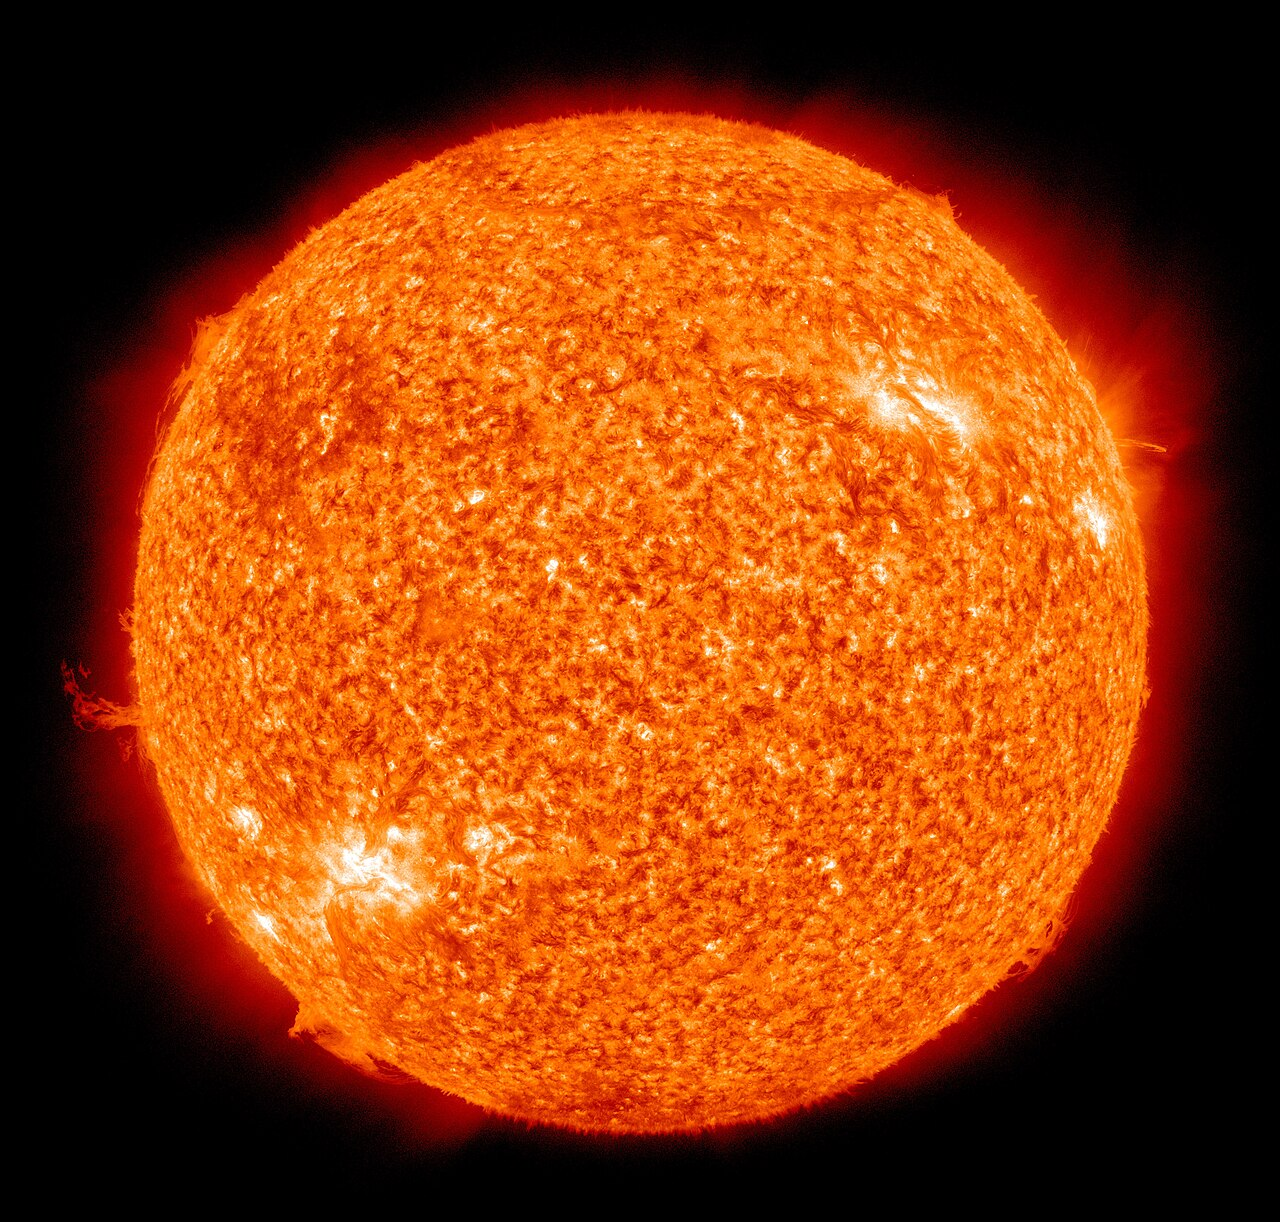
\includegraphics[width=0.4\linewidth]{images/book4/sun-sdo-aia.jpg}\hfill
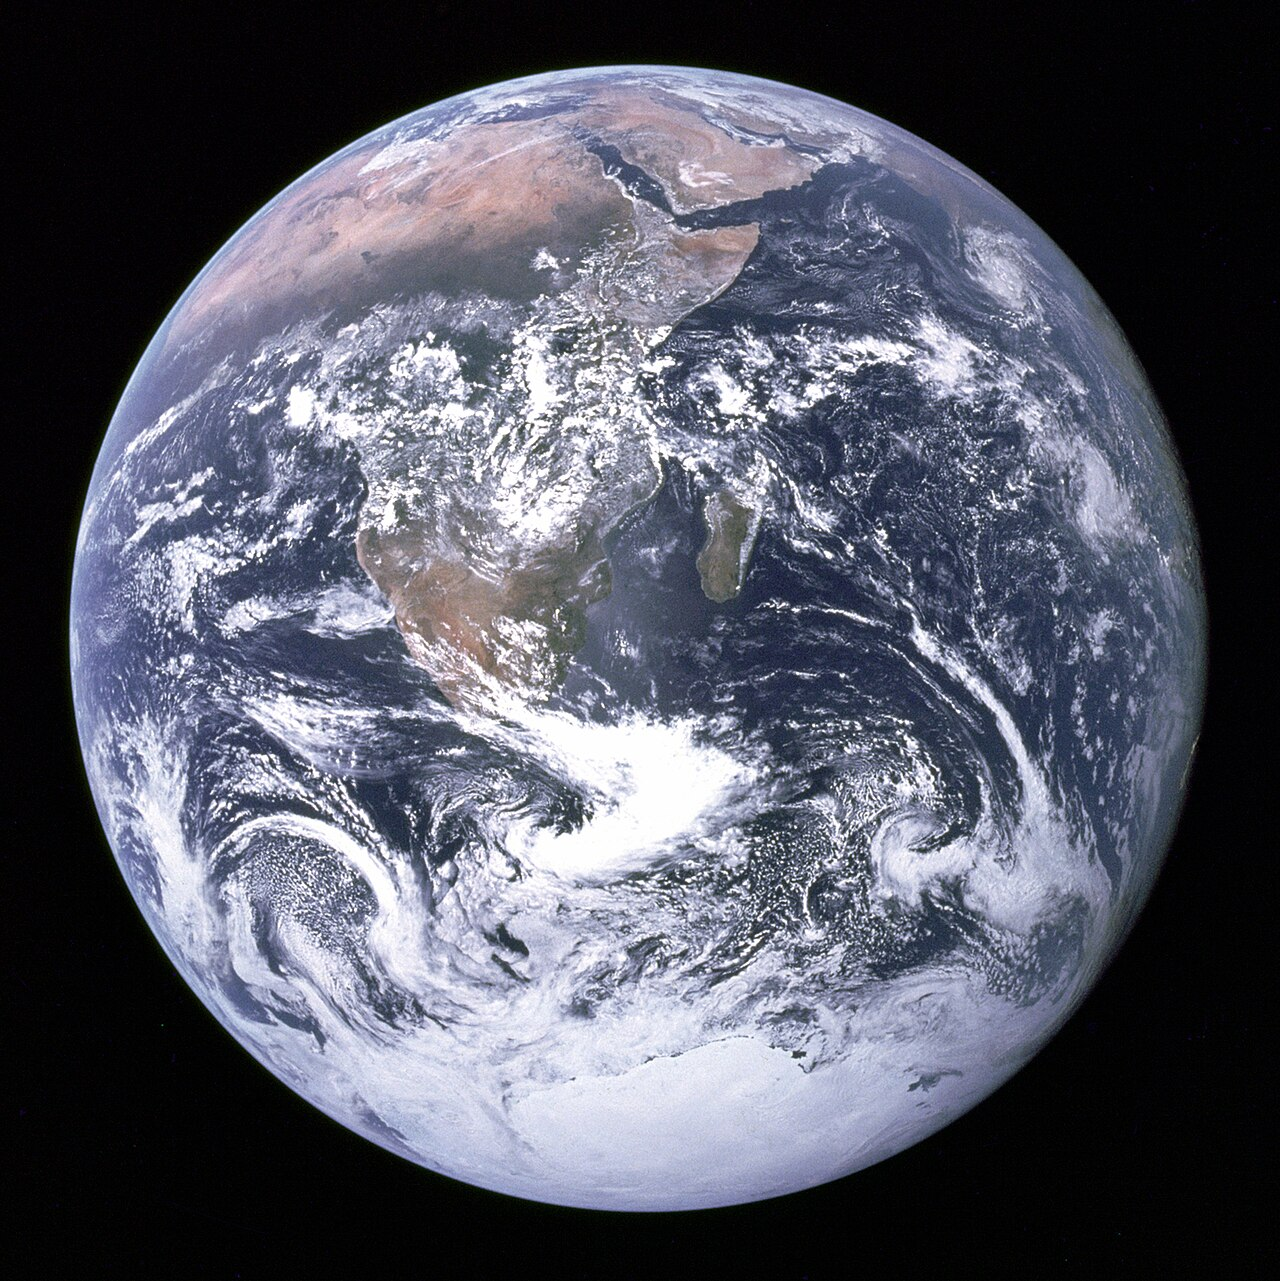
\includegraphics[width=0.4\linewidth]{images/book4/earth-apollo17.jpg}

{\small 本章的两个黑体：太阳（\qty{5800}{K}），由太阳动力学天文台在极紫外波段观测；地球（\qty{288}{K}），由阿波罗 17 号机组拍摄——峰值分别位于 \qty{0.5}{\micro m} 和 \qty{10}{\micro m}（NASA）。}
\end{omfigure}

\section{问题：地球的能量收支与白炽灯}

\begin{problem}[{周末问题——从太阳到
灯丝的黑体}]\label{pb:b2:thermal-radiation:1}
数据：$\sigma = \qty{5.67e-8}{W/m^2/K^4}$，$\lambda_{\max}T = \qty{2.90e-3}{m.K}$，
$h = \qty{6.63e-34}{J.s}$，$k_B = \qty{1.38e-23}{J/K}$，$c = \qty{3.00e8}{m/s}$；
太阳：$R_\odot = \qty{6.96e8}{m}$，$d = \qty{1.50e11}{m}$；地球：$R =
\qty{6.37e6}{m}$，反照率 $0.30$。

\textbf{第一部分——作为黑体的太阳。}
\begin{enumerate}
  \item 太阳光谱在 \qty{0.50}{\micro m} 处有峰值：表面
        温度。
  \item 表面的出射度与总光度。
  \item 地球处的太阳常数；
        此处日光的能量密度与压强。
  \item 平均光子能量（$\approx 2.7\,k_BT$）与
        地球处每秒每平方米的太阳光子数。
  \item 太阳以此速率辐射了 $4.5 \times 10^9$ 年：
        求辐射的总能量，并与 $Mc^2$ 比较，其中 $M = \qty{2e30}{kg}$。
\end{enumerate}

\textbf{第二部分——无大气层的地球。}
\begin{enumerate}[resume]
  \item 地球吸收的功率；有效温度。
  \item 平衡式为何要除以 $4$？
        对于不自转、无大气的地球，日下点
        的温度（$A = 0.30$）为多少？
  \item 月球（$A = 0.12$）：日下点温度；以及其夜侧
        为何降至 \qty{100}{K}（考虑两周白昼期间
        月壤所储存的热量，有效值取 \qty{1e6}{J/m^2/K}）。
  \item 地球发射峰的波长；与
        太阳的相比较。
  \item 若冰或云使反照率升至 $0.35$，
        有效温度将下降多少？
\end{enumerate}

\textbf{第三部分——温室效应。}
\begin{enumerate}[resume]
  \item 写出单层模型中三个平衡式（空间、大气层、地表），
        并由此得 $T_{\text{s}} = 2^{1/4}T_{\text{e}}$。
  \item 设大气层吸收红外线的比例为 $\varepsilon$：
        求 $T_{\text{s}}(\varepsilon)$，并求使其为
        \qty{288}{K} 的 $\varepsilon$ 值。
  \item 哪些气体吸收、哪些不吸收，以及
        吸收发生在哪些波段？大气窗口是什么？
  \item 大气向地面回送的红外辐射，
        单位为 \unit{W/m^2}，取 $\varepsilon = 0.78$ 模型；与
        被吸收的日光相比较。
  \item 强迫量为 \qty{3.7}{W/m^2}（二氧化碳加倍）：
        温度变化 $\Delta T = \Delta F/4\sigma T_{\text{e}}^3$
        （不计反馈）。
  \item 求厚 \qty{50}{m} 的海洋混合层单位面积的热容，
        以及响应的时间常数。
  \item 为何云既使地表降温（经反照率），又使其增温（经红外）；
        夜间哪一种效应占优？
\end{enumerate}

\textbf{第四部分——白炽灯。}
一只 \qty{60}{W} 的灯泡，其钨丝温度为 \qty{2800}{K}，
$\varepsilon = 0.35$；黑体功率中落入
可见光（$0.4$--\qty{0.7}{\micro m}）的份额在 \qty{2800}{K} 时为 $0.08$，
在 \qty{3200}{K} 时为 $0.14$。
\begin{enumerate}[resume]
  \item 灯丝的辐射面积；与其面积相同的
        线径为 \qty{50}{\micro m} 的导线长度；为何要卷成螺旋状？
  \item 峰值波长；可见光功率；发光效率。
  \item 在 \qty{230}{V} 电压下工作时灯丝的电阻；
        钨的电阻率在室温时约小十倍，
        求刚接通时的电流，并说明其后果。
  \item 在 \qty{3200}{K} 下：维持相同 \qty{60}{W} 所需的面积，
        以及可见光功率；为何不让每只灯泡都在 \qty{3200}{K} 下工作
        （钨的蒸发速率约每升高
        \qty{50}{K} 翻一番）？
  \item 卤素循环起什么作用？它为何允许
        灯丝温度更高？
  \item \qty{60}{W} 的其余部分去了哪里？灯泡玻璃
        为何能达到 \qty{150}{\celsius}？
  \item 断电后灯丝的冷却时间：由其质量
        （\qty{20}{mg}，$c = \qty{140}{J/kg/K}$）和辐射
        功率进行估算。
  \item 归纳：黑体的温度决定了什么，以及
        灯丝、太阳与地球有何共同之处。
\end{enumerate}
\end{problem}
